\newpage
\thispagestyle{empty}
\mbox{}

\chapter{Modelos de programación basados en paralelismo a nivel de tareas}
\label{ch:chapter3}

\section{Descripción general y estado del arte}

\section{OmpSs}

\subsection{Modelo de programación}

\subsection{Planificador de tareas}

\subsection{Ejemplo. Factorización de Cholesky}


\section{Adaptación de OmpSs a arquitecturas asimétricas (botlev)}
%%
\comentario{No se si adaptación, o ampliación, o incorporación, o uso de
  ompss sobre asim, o ...} %%
Con el reciente auge de las arquitecturas asimétricas en el mundo HPC, el
equipo de desarrollo de OmpSs ha introducido un nuevo planificador
denominado \emph{Bottom level-aware scheduler} (Botlev)~\cite{botlev}
específico para este nuevo tipo de arquitecturas. Botlev recoge las ideas
de los planificadores tradicionales basados en arquitecturas heterogéneas,
distinguiendo únicamente dos tipos de nodos de cómputo (un nodo rápido
formado por los cores de tipo big, y un nodo de cómputo lento formado por
los cores de tipo LITTLE) y eliminando el
cálculo de los costes asociados a la transferencia de datos. \\
La principal idea que se encuentra detrás de Botlev es la de detectar en
tiempo de ejecución qué tareas pertenecen al camino crítico y cuáles no, y
obligar a que los cores rápidos sean los encargados de ejecutar las tareas
del camino crítico. Además, en caso de existir alguna tarea perteneciente
al camino crítico lista para ser ejecutada, esta tendrá preferencia sobre
el resto de tareas que también estén listas para ejecución.\\
%%
\comentario{También se puede hablar de que botlev lo hace en tiempo de
  ejecución, por lo que no necesita conocer el problema de antemano, o usar
  oráculos, o asumir hechos.} %%
El objetivo de garantizar que las tareas del camino crítico se ejecutan en
los cores rápidos cuanto antes es asegurarse que al ejecutar las tareas
críticas, estas liberarán dependencias con nuevas tareas que pasarán a
estar listas para ejecución, y así intentar conseguir que nunca haya cores
ociosos, lo cual disminuiría el rendimiento global de la aplicación.

Para determinar si una tarea pertenece al camino crítico o no en tiempo de
ejecución, botlev asigna una prioridad a cada tarea en el momento de la
inserción en el grafo de dependencias. Una vez que la tarea está lista para
ser ejecutada (es decir, cuando todas las tareas que tenían relación con la
tarea mediante el grafo de dependencias han sido ejecutadas), se realiza la
decisión de qué core va a ejecutar la tarea en función de la prioridad
asignada.\\
La prioridad de una tarea viene dada por un número entero positivo, el cuál
representa la longitud del camino más largo desde la tarea actual hasta una
tarea hoja del grafo de dependencias. Cunado una tarea es introducida en el
grafo de dependencias, se le asigna una prioridad 0: la longitud del camino
más largo desde la tarea a un nodo hoja (ella misma) es 0. Además, cuando
una tarea se inserta, se actualizan las prioridades de todas las tareas
predecesoras, ya que esta puede haber cambiado. Por cada tarea predecesora,
se intenta aumentar la prioridad en 1 unidad (el camino es un nodo más
largo), siempre que no tuviera una prioridad mayor antes (este es el caso
de que la tarea pertenezca a un camino más largo en el que la tarea actual
no esté involucrada). El proceso de actualización finaliza cuando se
actualiza la tarea raíz del árbol, o cuando se alcanza una tarea que
pertenece a otro camino más largo que el actual. En la figura~\todo{fig} se
puede ver el camino crítico detectado para una aplicación que calcula la
factorización de Cholesky sobre una matriz dividida en $8\times8$
bloques. Hay que destacar que esta forma de calcular el camino crítico
detecta las tareas que pertenecen al camino más largo, pero eso no implica
que sean aquellas que van a consumir la mayor parte del tiempo. Para
calcular esto, sería necesario conocer de antemano las necesidades de cada
tarea, o ir almacenando resultados parciales de ejecución de manera
dinámica para tomar decisiones en el futuro.

%%
\comentario{La figura de las colas no se ve muy bien.} %%
\begin{figure}
  \centering
  \setlength{\fboxsep}{5pt}
  
  \begin{subfigure}{.45\textwidth}
    \centering
    \fbox{\includegraphics[width=.8\linewidth]{Figures/botlev-tdg.png}}
    \caption{Camino crítico en botlev para una Factorización de Cholesky de
      $8\times8$ bloques.}
    \label{s3:fig:botlev_tdg}
  \end{subfigure}
  % Si se deja una línea en blanco, las coloca en vertical
  \begin{subfigure}{.45\textwidth}
    \centering
    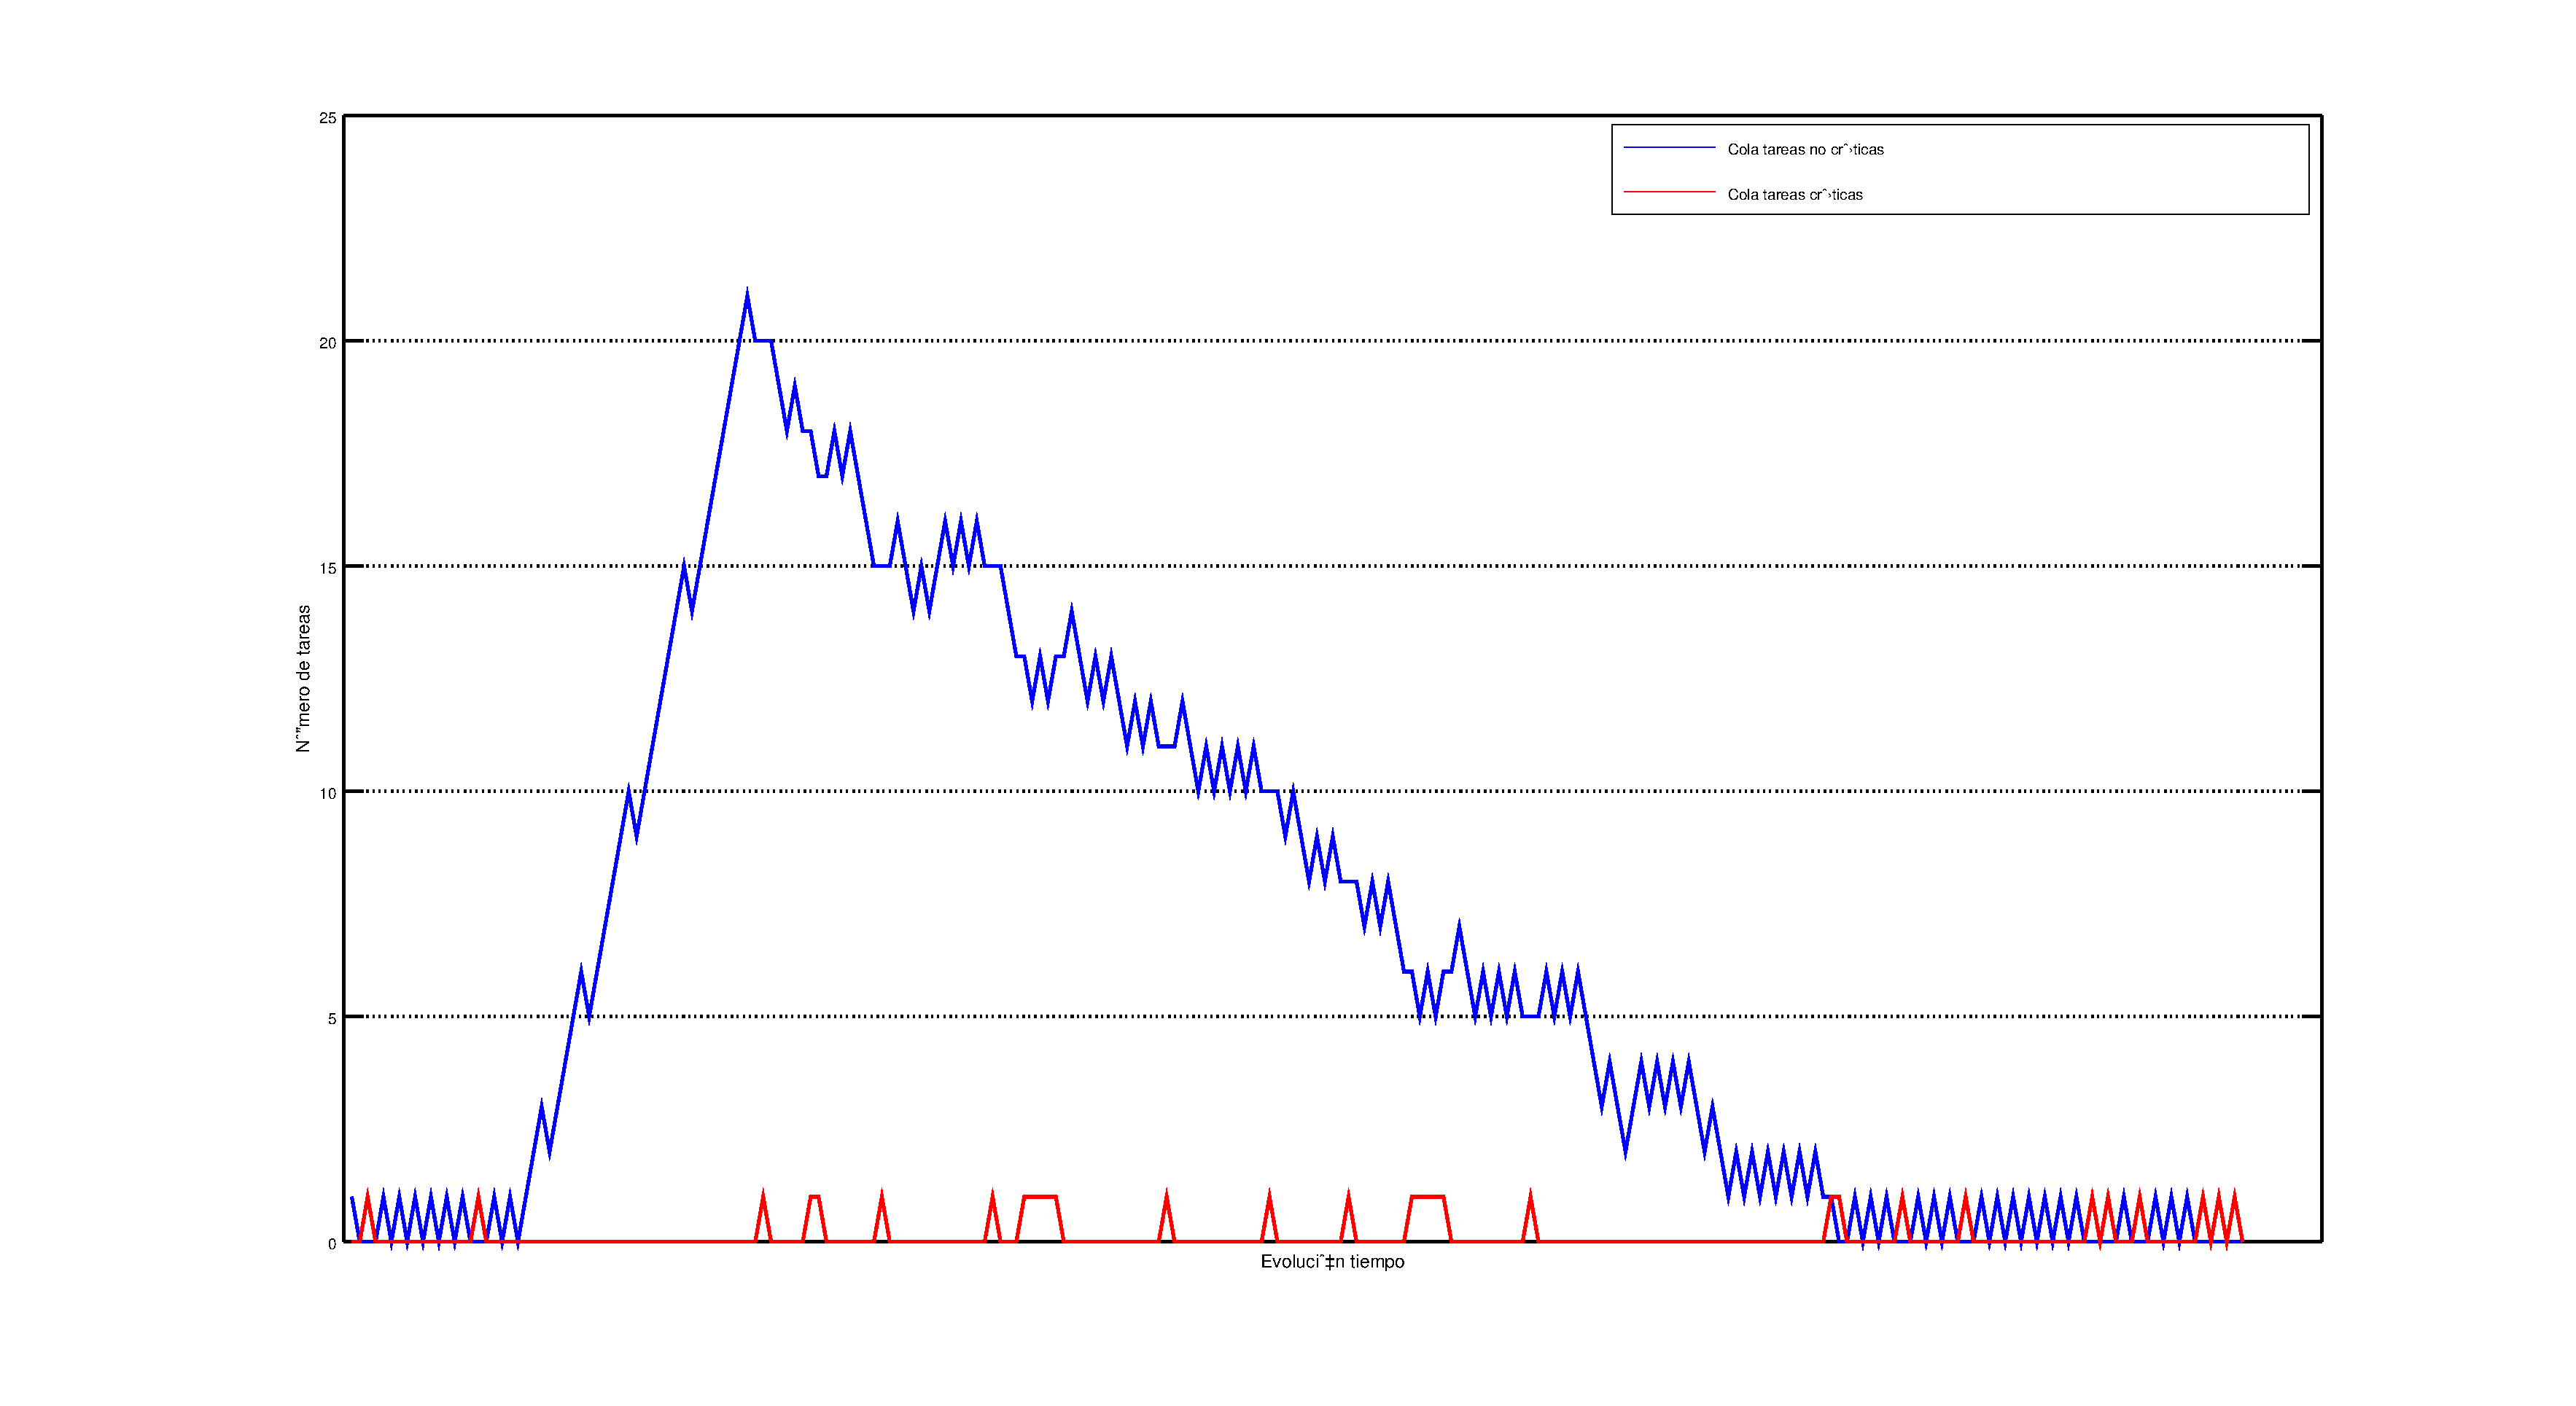
\includegraphics[width=1\linewidth]{Figures/botlev-colas.eps}
    \caption{Evolución de las colas de tareas listas.}
    \label{s3:fig:botlev_colas}
  \end{subfigure}  
  
  \caption{Cálculo de tareas críticas en Botlev y asignación a cores.}
  \label{s3:fig:botlev}
\end{figure}






%-- Configuraciones para emacs --
%%% Local Variables:
%%% mode: latex
%%% TeX-master: "./principal.tex"
%%% End:
